% Include Contributions page
\chapter{Plan of Work \& Project Management}

\section{Report Coordination}
\subsection{Breaking Up The Report}

Working in such a large team can be cumbersome at best at outright impossible
at worst when every person is a novice.  Knowing this, it was important to
identify strength and weaknesses early on, and based on the point system
provided by the Report 2 rubric, attempt to come up with an equal distribution
of work.  This report was divided in such a way that each team member member
could own a part of the report and a part of the project.  Going into Demo 1,
the goal is to provide the core functionality as individual pieces.\\

Here is a breakdown for our system specifications:\\

\begin{itemize}
\item{\textbf{Jesse Ziegler} - Jesse, being one of the most familiar with
finance took responsibility for defining things such as customer requirements
and assisted with interaction diagramming.}
\item{\textbf{Eric Jacob} - Eric was instrumental in helping design the database
schema, basic programming, design of Data Structures, and class diagramming.}
\item{\textbf{Chris Mancuso} - Chris assisted Eric in designing the class
diagrams, Jesses with interaction diagramming and other members in their tasks.}
\item{\textbf{Evan Arbeitman} - Evan worked with Eric, Jesse, and Chris in
developing the test designs as well as having input on interaction diagrams.}
\item{\textbf{David Karivalis} - David's strength is front-end design and for
that reason, he has worked on the UI spec as well as all the front-end
development.}
\item{\textbf{David Patrzeba} - David took on the project lead role and has been
driving the project forward ensuring that deadlines are met.  David has the most
programming experience and has acted as a technical advisor at every level of
the software stack.  He was instrumental in developing the algorithm that drives
the webapp.}
\end{itemize}

It's important to note that this does not perfectly represent each members
contributions, and that many sections had overlapping of team members. Sections
that involved mock-ups and diagrams in particular were developed by several
members overseen by the people given the responsibility as stated above.
Pieces of the report not mentioned above were worked on by multiple or all of
our members. The exact breakdown of contributions is impossible to describe. \\

\subsection{Compiling The Report}
In order to build this report a template was borrowed from a previous team to
quickly facilitate a professional style and presentation.  Compiling the report
was done using \LaTeX.  The key to presenting a consistent style across the
report was to have only one individual compile the report, while the rest of
the members concentrate on developing content for the report.  That does not
mean that one person had no content contributions, and 5 people had no styling
contributions, just that once the styling decisions were made, only one person
was allowed to compile the report.  All members acted as editors and revised
drafts of the report.  One area of inconsistency will be in the figures and
images, since different software was used by different members.

\subsection{Experiences}
 David Patrzeba asked each group member to explain their experience on the
 coordination of the report, any praise or criticism they had for the fellow
 members, and any issues that were encountered:

\subsubsection{Jesse Ziegler}

\subsubsection{Eric Jacob}
This project has been a different experience for me thus far.  Coming into this
class and this project, I expected to get more experience in programming, but I
feel that thus far in the project, it hasn't really been coding and its been a
lot of documentation.  However, from the experience that I've had before in
programming, I am able to see the connection (especially the system sequence
diagrams) between how the documentation relates to the coding.  The
documentation helps to give a clear view of what needs to be coded, what classes
need to be created, the different controllers that need to be created, etc.  In
this aspect, I feel like I've learned something that I haven't done before and
so it was useful.  Going forward, I really hope to sharpen my database design
skills through development of the database for our investment league, I hope to
become more familiar with user interface technologies as I don't have much
experience in that area, I also hope to learn some SCALA.  Lastly, I'd like to
learn some more about Object Oriented Design.  I hope to make a big contribution
to this project.

\subsubsection{Chris Mancuso}

\subsubsection{Evan Arbeitman}
Overall, working on this project has been a big learning experience thus far.
I've never worked with software on this scale, and I have been exposed to a lot
of new ideas and concepts that are essential to development, especially Git.
Although I'm new to Git, I've learned how powerful it is when it comes to
version control when working in a group of people with conflicting schedules.
Having a Git wiki page allows us to break up the work and keep track of
progress we've made. Also, as long as we are in constant communication, I know
our work as a group is efficient. One of my concerns moving forward would be my
ability to program in a language that I'm not completely familiar with. With
the help of David Patrzeba and Eric Jacob, I hope to learn more about Database
programming using MySQL; I just want to make sure I don't slow down our progress
over the next couple of weeks.

\subsubsection{David Karivalis}

\subsubsection{David Patrzeba}
I think that the group is coming along nicely, many of the members of the group
had little or no real world experience with medium sized software projects and
so bringing them up to speed has been a great experience.  This of course is
also an issue since it slows development, but we have been able to use this as
an advantage by boiling the project down to a minimal viable product and
concentrating on core aspects of the system.  Some tools that have helped
facilitate our groups progress have been Google+ hangouts for allowing us to
have project meetings without being co-located and to discuss technical issues
with one another, and Github and git source control which allows us to have multiple
versions of the project being developed all at once.  I have also learned much
about working team dynamics in software projects to accomplish end goals.\\

\section{Statement for Plan of Work}
For the remainder of this project, development of Paramount Investment League
will be divided into two major deliverables. The first deliverable will be a
an alpha release featuring a set of core functionality needed to deliver a
minimal viable product. This first deliverable is expected to be completed by
the last week in March. Following the completion of this milestone, the project
will be live in an alpha state at an undisclosed IP address with no search engine
indexing.  We will invite a set of users to use the product and provide feedback
and do in house user observations.  The goal is to see how users use the system
and see what they want the system to do in order to facilitate a better product.
This is very much in line with the Agile development methodology.\\

\section{First Deliverable (Demo 1)}
\subsection{Logic Implementation}
The logic of the first deliverable is further divided into subcomponents which
are the primary pillars of Paramount Investment League. \\
\subsubsection{1. Routing Scheme}
The Routing Scheme is developed and configured to allow our system to remain
in a stateless state, facilitate AJAX calls, and provide Comet frames for server
to client push.  This scheme does not have to be complete and can be modified
easily as more functionality is added. That said, care must be taken to ensure
that unnecessary functionality is not exposed, since once it is, by contract we
must continue to support it, otherwise we risk breaking functionality.\\
\subsubsection{2. Users}
Since the site is built around users, we have to ensure that their experience is
the best that we can make it.  To facilitate this, we have designed a system
that harnesses power of OpenID\cite{wiki:open} and OAuth\cite{wiki:oauth} and
allow users a no barrier registration process.  That is, using existing
credentials, users can log into Paramount Investment League without telling us
who they are.\\
\subsubsection{3. Leagues}
Leagues will be in a very early stage for the first development, and will mostly
be simply a proof of concept to provide user grouping.  These will be expanded
in demo 2 by allowing league creators to define goals for winning the league.
Every user will belong to the global league, which is the site wide tracking
of all users.  Leader boards will be calculated at the end of the trading day
and updated.\\
\subsubsection{4. Portfolios}
The portfolio is the center piece for the users interaction with the system.
Every user will be given a starter portfolio when they first register.  A user
also receives a new portfolio for every league they join.  As the system
progresses, league portfolios should be customizable, that is, they should be
able to be defined by the league manager.  We will try to implement this for
demo 2.\\
\subsection{User Experience}
The user experience is instrumental in driving new users to the website.  We
have attempted to make the system usable across multiple platforms by harnessing
modern technologies and platforms in order to deliver content across mobile,
tablet, and desktop.\\

\subsubsection{1. View Structure Finalization}
Using an MVC framework allows us to separate the view from the back end of the
system.  This allows us to ultimately customize views based on the device being
used.  In addition to targeting devices, we are using the Twitter Bootstrap
platform which is responsive and helps facilitate delivering content across
platform paradigms.
\subsubsection{2. Implement User Experience}
This is primarily the development of the look and feel of the web site.  This
will of course be iterated on and will not be a final version, but will be used
to retrieve feedback from our alpha users on how the website works for them, how
they wish it worked, and later making the necessary tweaks to facilitate this.\\
\subsubsection{3. AJAX Integration}
This is a key component of the front end calling into the back end in order to
give a seamless experience as the user navigates and uses the system.  By using
AJAX we avoid page refreshes for accomplishing tasks such making a trade.\\
\subsubsection{4. Comet Infinite Frames}
This may or may not make into demo 1, but we are trying our best to get it in.
Comet\cite{wiki:comt} allows the server to push data to the client in real time
and update the client page without the client making a request. To best describe
this, it is a reverse AJAX call.

\section{Second Deliverable (Demo 2)}
For both the logic and user experience sides of the system, the following
timeline of events applies. This timeline is slightly more malleable as
feedback quality/quantity can’t be accurately projected. \\

\subsubsection{1. Responding to feedback}
This is key to building our beta demo; demo 2; and finalizing the minimal viable
product, which involves nailing down the feature set, the initial user experience,
and a bug bash on edge cases discovered during the feedback phase.\\

\section{Breakdown of Responsibilities}
\subsubsection{Evan Arbeitman}
Evan will be leading the testing aspects of the system, including but not
limited to unit testing and integration testing. He will also be responsible
for developing and monitoring the feedback of the user base.\\
\subsubsection{Eric Jacob}
Eric will be leading the system administration and database scripting and
development of the system.  His responsibilities include developing the database
schema and keeping the hardware-software stack of developer and production
machines in sync.
\subsubsection{Chris Mancuso}
Chris will be assisting Eric in system administration duties as well as driving
the model construction which models the database schema in an object-oriented
paradigm, allowing us to (CRUD) create, read, update, and delete records in the
database.
\subsubsection{David Karivalis}
David's strength is in front-end development and for that reason he will be
driving the construction of our views and will be responsible for the user
experience.
\subsubsection{Jesse Ziegler}
Jesse will be primarily responsible for building controllers and assisting David
Karivalis in building the appropriate AJAX calls into the controller.  Jesse
will also be working closely with Chris to ensure that the interfaces exposed
by Chris's models are sufficient to accomplish the necessary tasks needed by
the views.
\subsubsection{David Patrzeba}
David has the most experience on the team and will be working across the entire
stack assisting every individual.  He is also responsible for developing the
core services that must run on the server. He is also responsible for performing
code reviews of all the code that goes into production and to help facilitate
the integration of all functionality.

\hfil\eject \pdfpagewidth=8.5in \pdfpageheight=11in
\begin{figure}
\section{Projected Milestones}
\centering
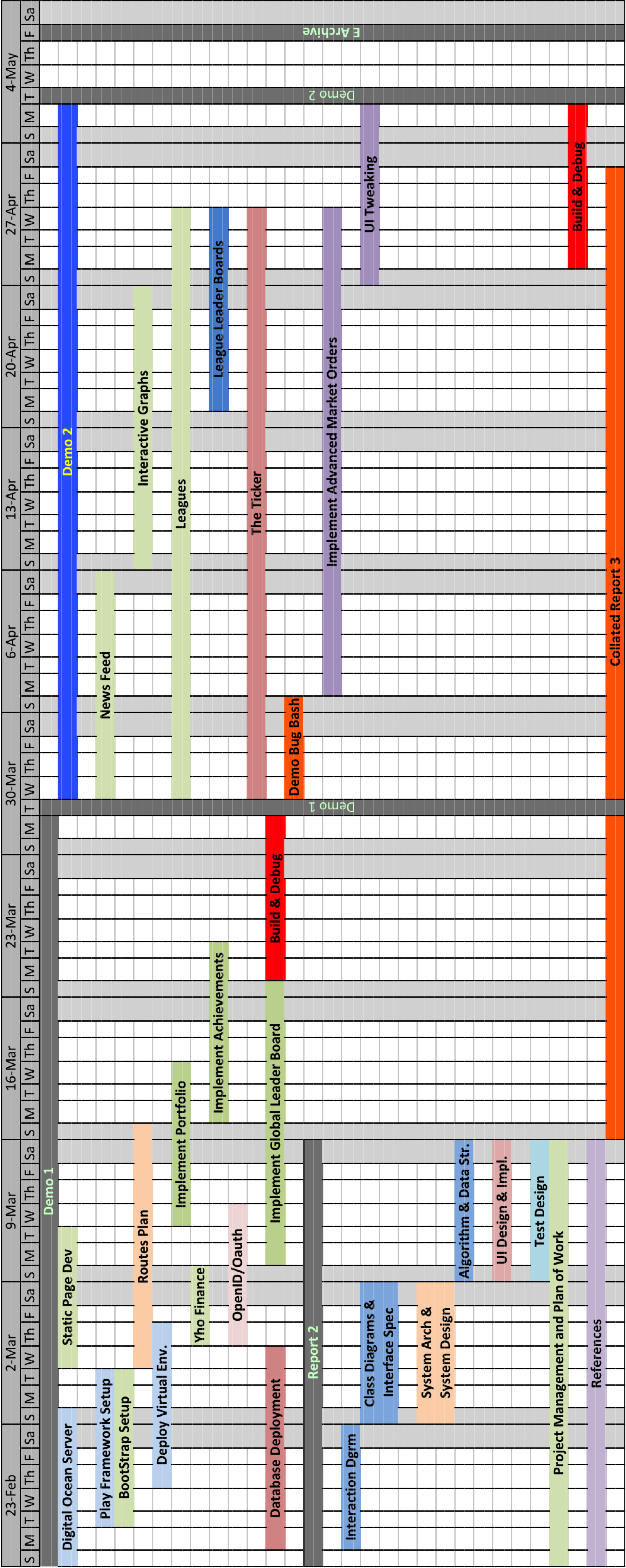
\includegraphics[height=9in]{./img/planOfWork.png}
\caption{This chart is the roadmap to meeting all our milestones.}
\end{figure}

%\section{User Story Matrix}
\section{Report 2 Contributions}

Report 2 was built as a team effort between all of team 1 and involved much
cross discussion in developing the report and the project.  For this reason we
feel that it is not possible to accurately weight the contributions and request
that each member receive an equal contribution.
